\section{Resultados}\label{sec:results}

\subsection{Verificación de componentes}\label{sec:res-verif}

La tabla~\ref{tab:verification} resume el estado de los componentes de la
cadena usada. De las \VerRows{} formulaciones del núcleo contrastadas por el
paquete con el manual de los autores del método \parencite{waters2002sebal},
\VerVerified{} están verificadas palabra por palabra, \VerCorroborated{}
corroboradas y \VerCandidate{} siguen como candidatas; el contraste detectó
\VerDiscrepancies{} discrepancias, \VerFixed{} de ellas corregidas en el
código. En este entorno de ejecución (R~4.3.3, \pkg{terra}~1.7-65) se
ejecutaron \NTests{} bloques de pruebas con \NExpectations{} expectativas:
\NTestsPassed{} bloques aprobados, \NTestsFailed{} fallos, \NTestsSkipped{}
omitidos por requerir dependencias opcionales y \NTestsError{} con error,
todos en la lectura de archivos HDF de MODIS por una incompatibilidad con
la versión local de \pkg{terra}; esa lectura no se usa en el estudio, que
parte de la escena ya preprocesada. Las pruebas de la cadena METRIC verifican
el cierre de energía en las anclas ($H = H_{target}$ con tolerancia relativa
$10^{-10}$), $LE = \Rnet - G - H$ en cada píxel y la reproducción de las
condiciones de borde de $\ETrF$; el núcleo GWR coincide con \pkg{GWmodel}
hasta $10^{-10}$. Dos componentes centrales de este estudio siguen como
candidatos: la transmisividad particionada de Allen y los criterios de
selección de anclas.

\begin{table}[htbp]
\centering\footnotesize
\caption{Componentes de la cadena METRIC usada, estado de verificación y
pruebas (fuente: \texttt{config/verification\_map.csv} y
\texttt{dev/VERIFICATION.md} del paquete).}\label{tab:verification}
\begin{tabularx}{\textwidth}{>{\raggedright\arraybackslash}p{3.4cm}>{\raggedright\arraybackslash}X>{\raggedright\arraybackslash}p{2.9cm}>{\raggedright\arraybackslash}p{3.1cm}r}
\toprule
Componente & Funciones & Estado & Fuente & Pruebas \\
\midrule
Radiación neta & \texttt{ef\_net\_radiation()} & VERIFICADA (SEBAL-Idaho 2002) & Waters et al. (2002), Ec. 2 & 63 \\
Onda corta incidente, terreno plano & \texttt{ef\_rs\_in(method = modelled)} & VERIFICADA (SEBAL-Idaho 2002) & Waters et al. (2002), Ec. 12 & 67 \\
Transmisividad particionada (Allen) & \texttt{ef\_tau\_sw(method = allen)} & CANDIDATA & ASCE-EWRI (2005), forma de Allen (1996) & 67 \\
Emisividad atmosférica & \texttt{ef\_atm\_emissivity()} & VERIFICADA (SEBAL-Idaho 2002) & Waters et al. (2002), Ec. 22 & 67 \\
Onda larga incidente y emitida & \texttt{ef\_rl\_in(), ef\_rl\_out()} & VERIFICADA (SEBAL-Idaho 2002) & Waters et al. (2002), Ecs. 20-23 & 67 \\
Flujo de calor del suelo (Bastiaanssen) & \texttt{ef\_g(method = bastiaanssen)} & VERIFICADA (SEBAL-Idaho 2002) & Waters et al. (2002), Ec. 24 & 39 \\
Flujo de calor del suelo (Tasumi) & \texttt{ef\_g(method = tasumi)} & CANDIDATA & Tasumi (2003) & 39 \\
Rugosidad por LAI & \texttt{ef\_zom(method = lai)} & VERIFICADA (SEBAL-Idaho 2002) & Waters et al. (2002), Ec. 31a & 15 \\
Viento a altura de mezcla y u* & \texttt{ef\_blending\_wind(), ef\_ustar()} & VERIFICADA (SEBAL-Idaho 2002) & Waters et al. (2002), Ecs. 27, 29, 30 & 15 \\
Resistencia aerodinámica y estabilidad & \texttt{ef\_rah(), psi\_m, psi\_h, L} & VERIFICADA (SEBAL-Idaho 2002) & Waters et al. (2002), Ecs. 26, 34-41 & 39 \\
Calibración dT y calor sensible & \texttt{ef\_calibrate\_h(), ef\_dt\_coef(), ef\_sensible\_heat()} & VERIFICADA (forma); procedimiento P0-10 & Waters et al. (2002), Ecs. 25, 32, 33 & 30 \\
Condiciones de borde de las anclas & \texttt{ef\_anchor\_conditions()} & VERIFICADA (forma) & Waters et al. (2002), p. 30-31 & 9 \\
Criterios de selección de anclas & \texttt{ef\_select\_anchors(), ef\_anchor\_criteria()} & CANDIDATA & Waters et al. (2002), ap. 7 & 28 \\
Calor latente, ET instantánea, ETrF y ETa diaria & \texttt{ef\_latent\_heat(), ef\_et\_inst(), ef\_etrf(), ef\_et\_daily()} & VERIFICADA (FAO-56; SEBAL-Idaho 2002) & Waters et al. (2002), Ecs. 1, 42-44 & 44 \\
ET de referencia ASCE-EWRI horaria & \texttt{ef\_ref\_et(), ef\_ref\_net\_radiation(), ef\_ref\_soil\_heat\_flux()} & VERIFICADA (ecuaciones y constantes) & ASCE-EWRI (2005) & 58 \\
Regionalización C1/C2/C3 y núcleo GWR & \texttt{ef\_regionalize(), ef\_regionalize\_cv(), ef\_gwr\_*()} & CANDIDATA (corroborada con GWmodel a 1e-10) & Brunsdon et al. (1996); Gollini et al. (2015) & 75 \\
\bottomrule
\end{tabularx}

\end{table}

\subsection{Regionalización meteorológica}\label{sec:res-reg}

La regla D-02 seleccionó como estación representativa
\emph{\RepStationName}, a \RepStationDist{}~km del centroide de la provincia: la estación más
cercana con registros completos de temperatura, humedad y viento. La validación
cruzada espacial (\NFolds{} pliegues, \NCVDays{} días, \num[round-precision=0]{\NCVPred}
predicciones fuera de muestra) entregó los errores de la tabla~\ref{tab:cv}
y la figura~\ref{fig:cv}.

Para la temperatura del aire, todas las alternativas espaciales superaron a
la estación representativa (RMSE C1 = \CVTaCOneRmse{}~\si{\celsius},
IC~95\,\% [\CVTaCOneRmseLo; \CVTaCOneRmseHi]). La corrección por gradiente
vertical no mejoró a C1 (C1-lap: \CVTaCOneLapRmse{}~\si{\celsius}), lo que
indica que la diferencia entre la estación y el resto del territorio no es
principalmente altitudinal. GWR (\CVTaCThreeGWRRmse{}~\si{\celsius}
[\CVTaCThreeGWRRmseLo; \CVTaCThreeGWRRmseHi]) superó a C1 y a la regresión
global (\CVTaCTwoOLSRmse{}~\si{\celsius}); en la comparación pareada, su error
cuadrático fue menor que el de C1 en \PairTaCOneDse{}~\si{\celsius\squared}
en promedio (IC [\PairTaCOneLo; \PairTaCOneHi]) y que el de C2-OLS en
\PairTaCTwoOLSDse{}~\si{\celsius\squared} ([\PairTaCTwoOLSLo; \PairTaCTwoOLSHi]).
Sin embargo, el método de menor error fue IDW (\CVTaCTwoIDWRmse{}~\si{\celsius}
[\CVTaCTwoIDWRmseLo; \CVTaCTwoIDWRmseHi]): la diferencia pareada GWR$-$IDW fue
positiva, \PairTaCTwoIDWDse{}~\si{\celsius\squared} (IC
[\PairTaCTwoIDWLo; \PairTaCTwoIDWHi]), y GWR tuvo menor error absoluto que IDW
solo en el \PairTaCTwoIDWShare\,\% de las predicciones. El patrón se repite
para la presión de vapor: IDW (\CVEaCTwoIDWRmse{}~kPa) $<$ GWR
(\CVEaCThreeGWRRmse{}~kPa) $<$ OLS (\CVEaCTwoOLSRmse{}~kPa) $<$ C1
(\CVEaCOneRmse{}~kPa), con la diferencia GWR$-$IDW también positiva
([\PairEaCTwoIDWLo; \PairEaCTwoIDWHi]~\si{\kilo\pascal\squared}). Los sesgos
medios fueron pequeños para todos los métodos espaciales ($|$sesgo$|$ $\le$
\num{0.05}~\si{\celsius}).

Los residuos de C1 y de la regresión global conservaron dependencia
espacial (I de Moran mediano \MoranTaCOneI{} y \MoranTaCTwoOLSI{} para la
temperatura, significativo en el \MoranTaCOneSig\,\% y \MoranTaCTwoOLSSig\,\%
de los instantes), mientras que IDW y GWR la eliminaron casi por completo
(\MoranTaCTwoIDWSig\,\% y \MoranTaCThreeGWRSig\,\% de instantes
significativos). La densidad de la red condicionó a GWR más que a IDW
(figura~\ref{fig:density}): con \DensTaCThreeGWRQuarterN{} estaciones (25\,\%)
el RMSE de la temperatura fue \DensTaCThreeGWRQuarter{}~\si{\celsius} con GWR y
\DensTaCTwoIDWQuarter{}~\si{\celsius} con IDW, frente a \DensTaCThreeGWRAll{} y
\DensTaCTwoIDWAll{}~\si{\celsius} con la red completa.

El viento solo se mide en \NStationsWind{} estaciones. Con ellas, GWR no pudo
ajustarse en ninguno de los \CVWindCThreeGWRTotal{} casos de validación
(sin ancho de banda factible), y la regresión global produjo predicciones
fuera del dominio físico (máximo \CVWindOLSMax{}~\si{\metre\per\second};
\CVWindOLSNeg{} predicciones negativas) con RMSE de
\CVWindCTwoOLSRmse{}~\si{\metre\per\second}, frente a \CVWindCOneRmse{} de C1
y \CVWindCTwoIDWRmse{}~\si{\metre\per\second} de IDW.

\begin{figure}[htbp]
\centering
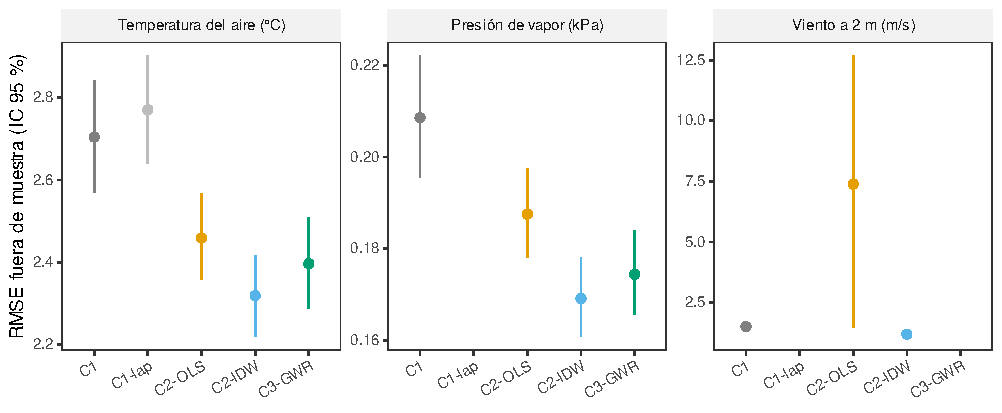
\includegraphics[width=\textwidth]{fig03_cv_rmse.pdf}
\caption{RMSE fuera de muestra (validación cruzada espacial anidada) por
variable y configuración, con IC~95\,\% por \emph{bootstrap} de días. GWR del
viento no fue factible (sin punto).}\label{fig:cv}
\end{figure}

\begin{table}[htbp]
\centering
\footnotesize
\caption{Validación cruzada espacial anidada de la regionalización a la hora del paso (14:00 UTC, enero--marzo de 2019).}\label{tab:cv}
\begin{threeparttable}
\begin{tabular}{llrlrlrr}
\toprule
Variable & Config. & $n$ & RMSE [IC 95\,\%] & MAE & Sesgo [IC 95\,\%] & $r$ & Fallidas \\
\midrule
$T_a$ (\si{\celsius}) & C1 & 5498 & 2,70 [2,57; 2,84] & 2,10 & -0,16 [-0,38; 0,07] & 0,70 & 0 \\
 & C1-lap & 5498 & 2,77 [2,64; 2,90] & 2,17 & -0,05 [-0,27; 0,18] & 0,68 & 0 \\
 & C2-OLS & 5588 & 2,46 [2,36; 2,57] & 1,92 & -0,01 [-0,02; 0,00] & 0,75 & 0 \\
 & C2-IDW & 5588 & 2,32 [2,22; 2,42] & 1,83 & 0,01 [-0,01; 0,03] & 0,78 & 0 \\
 & C3-GWR & 5588 & 2,40 [2,29; 2,51] & 1,85 & -0,04 [-0,07; -0,02] & 0,76 & 0 \\
$e_a$ (\si{\kilo\pascal}) & C1 & 5495 & 0,209 [0,195; 0,222] & 0,153 & -0,024 [-0,043; -0,005] & 0,69 & 0 \\
 & C2-OLS & 5585 & 0,188 [0,178; 0,198] & 0,135 & 0,003 [0,002; 0,004] & 0,73 & 0 \\
 & C2-IDW & 5585 & 0,169 [0,161; 0,178] & 0,120 & -0,005 [-0,006; -0,003] & 0,79 & 0 \\
 & C3-GWR & 5585 & 0,174 [0,166; 0,184] & 0,122 & -0,002 [-0,004; 0,000] & 0,77 & 0 \\
$u_2$ (\si{\metre\per\second}) & C1 & 505 & 1,51 [1,37; 1,64] & 1,20 & 0,63 [0,46; 0,80] & 0,52 & 0 \\
 & C2-OLS & 595 & 7,39 [1,48; 12,69] & 1,57 & 0,10 [-0,22; 0,70] & 0,08 & 0 \\
 & C2-IDW & 595 & 1,19 [1,10; 1,29] & 0,91 & -0,04 [-0,06; -0,02] & 0,58 & 0 \\
 & C3-GWR & 0 & \multicolumn{4}{l}{no factible (sin ancho de banda factible)} & 595 \\
\bottomrule
\end{tabular}
\begin{tablenotes}\footnotesize
\item $n$: predicciones fuera de muestra. Sesgo = predicho $-$ observado. IC: \emph{bootstrap} de días completos ($B = 2000$).
\item C1 no se evalúa en su propia estación. Fallidas: predicciones cuyo pliegue no pudo ajustarse con las estaciones de entrenamiento (p.\,ej., GWR o regresión global con menos estaciones que parámetros + 3).
\end{tablenotes}
\end{threeparttable}
\end{table}


\begin{figure}[htbp]
\centering
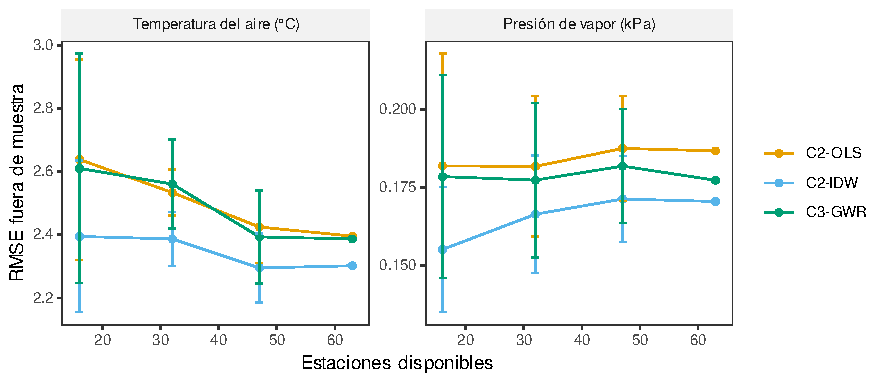
\includegraphics[width=0.85\textwidth]{fig09_density.pdf}
\caption{RMSE de validación cruzada según la fracción de estaciones
disponible (media de 10 subconjuntos aleatorios en 30 días; la barra indica
$\pm 1$ desviación estándar).}\label{fig:density}
\end{figure}

\subsection{Campos meteorológicos y balance de energía superficial}\label{sec:res-eb}

A la hora del paso, la escena recibió de C1 un valor único de temperatura
(\MFTaCOneMean~\si{\celsius}), presión de vapor (\MFEaCOneMean~kPa) y viento
(\MFWindCOneMean~\si{\metre\per\second}). Las configuraciones espaciales
produjeron campos con medias y amplitudes distintas
(figura~\ref{fig:forcing}): la temperatura media fue \MFTaCTwoIDWMean~\si{\celsius}
(DE espacial \MFTaCTwoIDWSd) con IDW y \MFTaCThreeGWRMean~\si{\celsius}
(DE \MFTaCThreeGWRSd) con GWR. El campo de GWR presentó máximos locales de
hasta \RangeTaCThreeGWRMax~\si{\celsius} en la Cordillera de la Costa, por
encima del máximo observado en las estaciones a esa hora
(\RangeTaCThreeGWRObsMax~\si{\celsius}) en el \RangeTaCThreeGWRAbove\,\% de
las celdas procesadas: los coeficientes locales se extrapolan en terreno sin
estaciones, un problema que la validación cruzada en las estaciones no puede
detectar. Ninguna otra configuración salió del rango observado. La $\ETr^{24}$
media de la escena fue \MFEtrDayCOneMean~mm/d con C1, \MFEtrDayCThreeGWRMean~mm/d
con GWR, \MFEtrDayCTwoIDWMean~mm/d con IDW y \MFEtrDayCTwoOLSMean~mm/d con la
regresión global. Estos resultados confirman H1: las configuraciones
producen diferencias espaciales identificables en las variables que entran
en METRIC (salvo el viento de GWR, que no fue factible).

\begin{figure}[htbp]
\centering
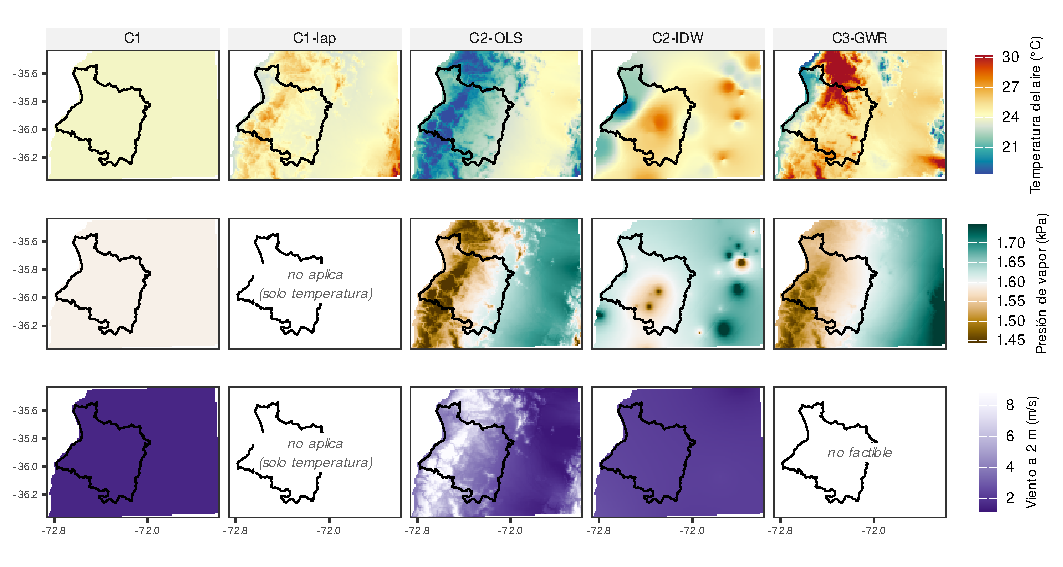
\includegraphics[width=\textwidth]{fig04_forcing_maps.pdf}
\caption{Temperatura del aire, presión de vapor y viento a 2~m regionalizados
a las 14:00~UTC del 15-02-2019 por configuración (grilla UTM~18S de 1~km;
mostrados en coordenadas geográficas). El viento de C3-GWR se reemplazó por
el de C1 (D-14).}\label{fig:forcing}
\end{figure}

Las celdas ancla fueron idénticas en \NRunsSameAnchors{} de las \NRuns{}
corridas; la excepción es C2-OLS, cuyo dominio válido se redujo a
\num[round-precision=0]{\OLSValidCells} celdas porque el viento regionalizado
salió del dominio físico, de modo que sus anclas se seleccionaron dentro de
ese dominio y C2-OLS no es comparable con el resto. Los cambios del forzamiento se tradujeron en cambios de la
calibración: $b$ varió entre \CalCThreeGWRB{} (GWR) y \CalCTwoIDWB{} (IDW) y
$a$ entre \CalCThreeGWRA{} y \CalCTwoIDWA~K (tabla~\ref{tab:metric}). La
radiación neta media aumentó \DRnCThreeGWRMean~\si{\watt\per\square\metre}
con GWR respecto de C1 (\MRnCOneMean{} frente a \MRnCThreeGWRMean~\si{\watt\per\square\metre})
y el calor sensible \DHCThreeGWRMean~\si{\watt\per\square\metre} (P5--P95:
\DHCThreeGWRLo{} a \DHCThreeGWRHi), de modo que el calor latente instantáneo
casi no cambió (\MLECOneMean{} frente a \MLECThreeGWRMean~\si{\watt\per\square\metre})
y la fracción $\ETrF$ media tampoco (\MEtrfCOneMean{} frente a
\MEtrfCThreeGWRMean; diferencia \DEtrfCThreeGWRPct\,\%). Con IDW, cuyo campo
de viento difiere del de C1, $\ETrF$ disminuyó \DEtrfCTwoIDWPct\,\%. La
figura~\ref{fig:eb} muestra los cuatro flujos por configuración.

\begin{table}[htbp]
\centering
\footnotesize
\caption{Balance de energía y $\mathrm{ET_a}$ de la escena de Cauquenes (15-02-2019) por configuración: media (desviación estándar espacial) y parámetros de calibración.}\label{tab:metric}
\begin{threeparttable}
\begin{tabular}{lrrrrr}
\toprule
Variable & C1 & C1-lap & C2-OLS & C2-IDW & C3-GWR \\
\midrule
$R_n$ & 475 (55) & 477 (56) & 449 (62) & 478 (49) & 483 (54) \\
$G$ & 58 (15) & 59 (15) & 66 (10) & 59 (16) & 59 (15) \\
$H$ & 267 (73) & 266 (74) & 325 (31) & 278 (79) & 271 (72) \\
$LE$ & 149 (135) & 153 (137) & 58 (87) & 140 (133) & 152 (132) \\
$\mathrm{ET_rF}$ & 0,40 (0,36) & 0,40 (0,37) & 0,15 (0,23) & 0,37 (0,38) & 0,40 (0,37) \\
$\mathrm{ET_a}$ (mm/d) & 3,45 (3,12) & 3,54 (3,17) & 1,04 (1,51) & 2,48 (2,26) & 2,76 (2,25) \\
$\mathrm{ET_r^{24}}$ (mm/d) & 8,56 (0,01) & 8,72 (0,26) & 6,95 (0,30) & 7,38 (0,86) & 7,56 (0,85) \\
\midrule
$a$ (K) & -65,73 & -67,00 & -30,77 & -73,83 & -64,94 \\
$b$ (--) & 0,231 & 0,236 & 0,115 & 0,258 & 0,229 \\
Iteraciones & 9 & 9 & 6 & 7 & 9 \\
$\mathrm{ET_r}$ inst. ancla fría (mm/h) & 0,544 & 0,554 & 0,563 & 0,535 & 0,535 \\
$u_{200}$ ancla fría (m/s) & 2,99 & 2,99 & 8,69 & 4,65 & 2,99 \\
Celdas con $\mathrm{ET_a} < 0$ & 77 & 74 & 156 & 102 & 58 \\
\bottomrule
\end{tabular}
\begin{tablenotes}\footnotesize
\item Flujos en \si{\watt\per\square\metre}. Las celdas ancla son las mismas en todas las configuraciones.
\end{tablenotes}
\end{threeparttable}
\end{table}


\begin{figure}[htbp]
\centering
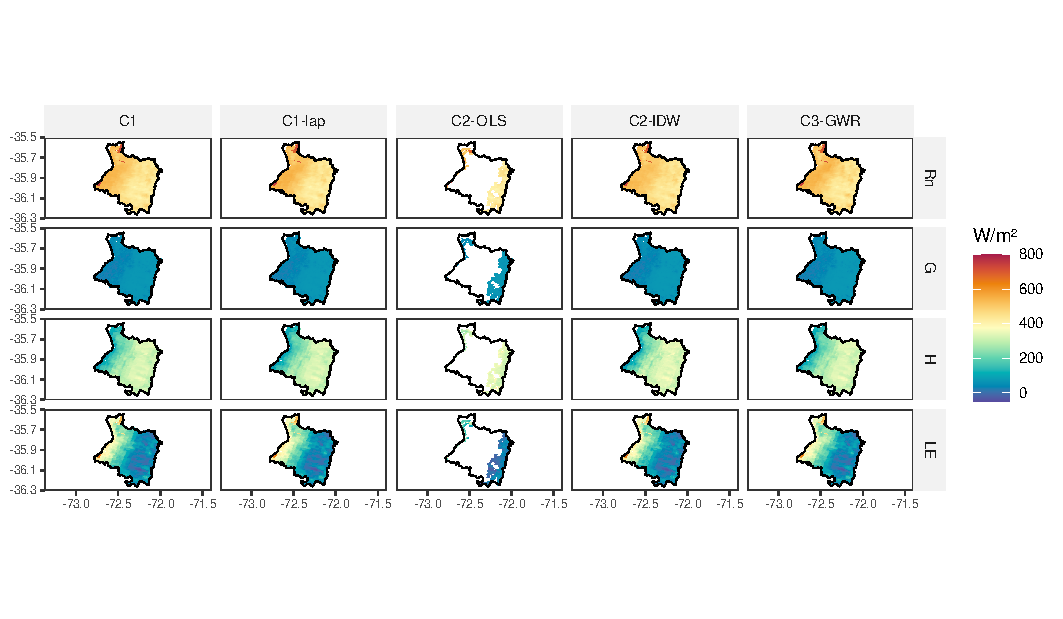
\includegraphics[width=\textwidth]{fig05_energy_balance.pdf}
\caption{Radiación neta, flujo de calor del suelo, calor sensible y calor
latente instantáneos (\si{\watt\per\square\metre}) por configuración.
C2-OLS tiene celdas sin datos donde el viento regionalizado salió del
dominio físico.}\label{fig:eb}
\end{figure}

\subsection{Evapotranspiración real}\label{sec:res-eta}

La $\ETa$ media de la escena fue \MEtaCOneMean~mm/d con C1,
\MEtaCOneLapMean~mm/d con C1-lap, \MEtaCTwoIDWMean~mm/d con IDW,
\MEtaCThreeGWRMean~mm/d con GWR y \MEtaCTwoOLSMean~mm/d con la regresión
global, esta última sobre solo \num[round-precision=0]{\OLSValidCells} celdas
válidas (figura~\ref{fig:eta}). Frente a C1, GWR redujo la $\ETa$ media en
\DEtaCThreeGWRMean~mm/d (\DEtaCThreeGWRPct\,\%), con diferencias locales
entre \DEtaCThreeGWRLo{} y \DEtaCThreeGWRHi~mm/d (P5--P95) y
$|\Delta\ETa| > 0{,}5$~mm/d en el \DEtaCThreeGWRShare\,\% de las celdas; IDW la
redujo en \DEtaCTwoIDWMean~mm/d (\DEtaCTwoIDWPct\,\%). La correlación espacial
entre los mapas fue alta (el patrón relativo se conserva), por lo que las
configuraciones cambian sobre todo el nivel y la amplitud de $\ETa$, no su
estructura.

La sustitución de una variable por vez (figura~\ref{fig:attr}) muestra que
el efecto no es uniforme entre vías de entrada (H2). La $\ETr^{24}$
regionalizada explicó casi todo el cambio: por sí sola modificó la $\ETa$
en \DEtaOatEtrDayMean~mm/d (\DEtaOatEtrDayPct\,\%). La $\ETr$ instantánea,
que actúa a través de la condición del ancla fría, cambió la calibración
($a$ = \CalOatEtrInstA~K; $b$ = \CalOatEtrInstB) con un efecto medio de
\DEtaOatEtrInstMean~mm/d y compensaciones locales (P5--P95:
\DEtaOatEtrInstLo{} a \DEtaOatEtrInstHi~mm/d). La temperatura del aire
contribuyó \DEtaOatTaMean~mm/d, la presión de vapor \DEtaOatEaMean~mm/d y el
viento (campo IDW, D-16) \DEtaOatWindMean~mm/d. Sin el viento, que en la
corrida conjunta de GWR es el de C1, la suma de los efectos individuales
($T_a$, $e_a$, $\ETr$ instantánea y $\ETr^{24}$) es prácticamente igual al
efecto conjunto (\DEtaCThreeGWRMean~mm/d): en esta escena, los efectos son
aproximadamente aditivos. En síntesis, la calibración interna absorbió casi
por completo el efecto del forzamiento sobre el balance instantáneo, y la
diferencia de $\ETa$ entró por la extrapolación diaria.

\begin{figure}[htbp]
\centering
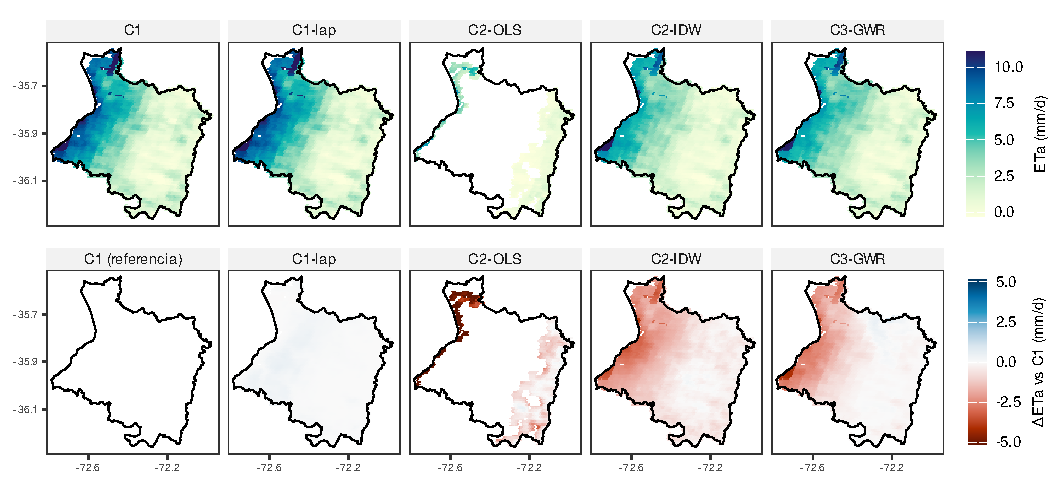
\includegraphics[width=\textwidth]{fig06_eta_maps.pdf}
\caption{Arriba: $\ETa$ diaria (mm/d) por configuración. Abajo: diferencia
respecto de C1 (mm/d). Escala común; valores fuera del rango P1--P99
saturados.}\label{fig:eta}
\end{figure}

\begin{figure}[htbp]
\centering
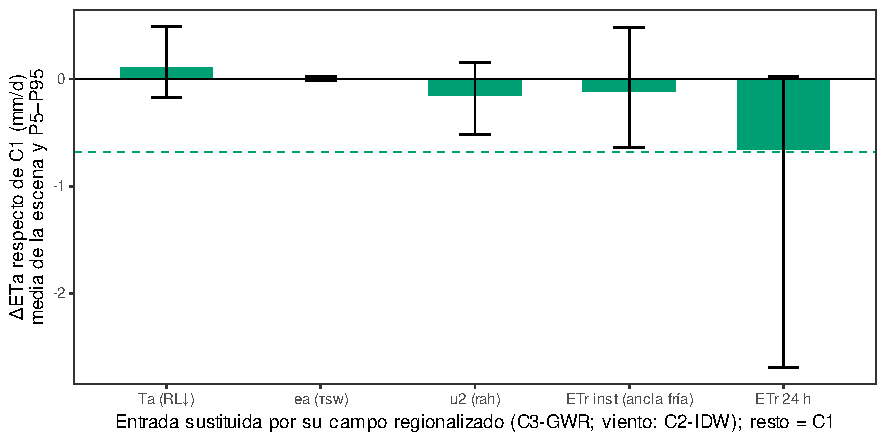
\includegraphics[width=0.8\textwidth]{fig07_attribution.pdf}
\caption{Cambio de la $\ETa$ media de la escena al reemplazar una sola
entrada de C1 por su campo regionalizado (C3-GWR; viento: C2-IDW). Barras de
error: P5--P95 de las diferencias por celda. Línea discontinua: sustitución
completa por C3-GWR.}\label{fig:attr}
\end{figure}

\subsection{Validación independiente}\label{sec:res-val}

No se dispuso de mediciones independientes de $\ETa$ o de flujo de calor
latente para el área y la fecha (sección~\ref{sec:validation-data}). Por lo
tanto, no se calcularon métricas de exactitud de $\ETa$ y \textbf{ninguna de
las diferencias anteriores puede interpretarse como mejora o deterioro de la
exactitud}. La única validación independiente del estudio es la de las
variables meteorológicas (sección~\ref{sec:res-reg}), evaluada fuera de
muestra en \NCVDays{} días.

\subsection{Sensibilidad y robustez}\label{sec:res-sens}

Las \NMC{} réplicas de criterios de anclas y condiciones de borde (S-A)
produjeron una dispersión de la $\ETa$ media de la escena de
\SACOneSd~mm/d (DE) con el forzamiento C1 y \SACThreeGWRSd~mm/d con GWR; el
ruido de los insumos MODIS (S-B) produjo \SBCOneSd{} y \SBCThreeGWRSd~mm/d,
respectivamente (figura~\ref{fig:sens}). En cada réplica, la diferencia
pareada GWR$-$C1 se mantuvo: \SAEffMean~mm/d (P2,5--P97,5:
\SAEffLo{} a \SAEffHi) bajo S-A y \SBEffMean~mm/d (\SBEffLo{} a \SBEffHi) bajo
S-B, con el mismo signo en el \SAEffSign\,\% y \SBEffSign\,\% de las réplicas.
Las alternativas estructurales (S-C) modificaron la $\ETa$ media de C1 de
\SCBaseCOne{} a \SCgTasumiCOne~mm/d (G de Tasumi), \SCZomFloorCOne~mm/d (piso
de rugosidad de 0,01~m) y \SCAggregateMeanCOne~mm/d (anclas por media). El ruido de LST desplazó hacia arriba la $\ETa$ media de C1
(intervalo \SBCOneLo--\SBCOneHi~mm/d frente a \SCBaseCOne~mm/d sin ruido), porque
la selección de anclas por extremos de LST es sensible al ruido por píxel. Todas
las calibraciones convergieron (\SACOneConv\,\% y \SBCOneConv\,\% de las
réplicas).

\begin{figure}[htbp]
\centering
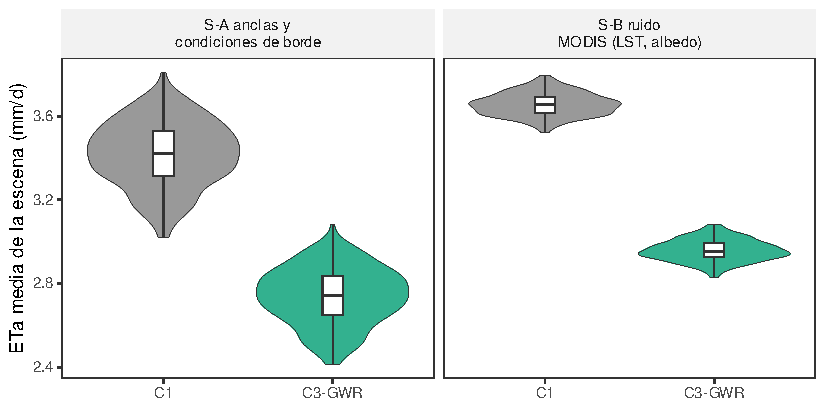
\includegraphics[width=0.85\textwidth]{fig08_sensitivity.pdf}
\caption{Distribución de la $\ETa$ media de la escena en \NMC{} réplicas
Monte Carlo de los criterios de anclas y condiciones de borde (S-A) y del
ruido de los insumos MODIS (S-B), con los forzamientos C1 y
C3-GWR.}\label{fig:sens}
\end{figure}
